\section{Modeling and MiL testing}\label{sec:modeling-for-mil-testing}

This section describes the power system model that will be used to demonstrate the application of eFMI to both synthesis and deployment of the controller code. The system to be modeled is illustrated in Figure \ref{fig:overview}, which shows a power plant interconnected to a power grid. The power plant's generator, a synchronous machine, is equipped with a PSS that is placed before the Excitation Control System (ECS). 

\begin{figure}[t!]
\centerline{\includesvg[width=0.975\columnwidth]{./figures/f01-overview-w.svg}}
    \caption{Diagram of a power plant's electrical generator equipped with a PSS interconnected with a power grid.}
    \label{fig:overview}
    \vspace{-0.1in}
\end{figure}

The main purpose of the ECS is to supply the exciter with sufficient excitation current and voltage, $v_f(t)$, to control the terminal voltage, $V_t(t)$, with respect to a reference value, $v_\mathrm{ref}(t)$, forming what is typically called the ``voltage control loop'' of the plant. The PSS uses the generator's speed, $\omega(t)$, as a feedback signal and is placed in a cascade with the ECS. This increases the damping of the plant's response through the effect of the positive feedback signal, $v_s(t)$. 

The goal of the PSS is to provide adequate damping and ensure the stability of the connection to the grid (in this case, a single power plant), or an entire interconnected region, when the grid is subject to disturbances, $d(t)$, such as faults, tripping of power lines, etc. However, to achieve this goal, these damping controllers must be properly tuned; if left without frequent tuning, they may lead to major grid stability problems, as described in the introduction. The PSS structure (a transfer function) is fixed, and the values of its parameters must be set through design studies before being implemented in the field.

\paragraph{Conventions:} Referring to Figure \ref{fig:overview}, we will use the term \controller{} to refer to the PSS, the term \generatorunit{} to refer to the generator and the ECS sub-system (with or without a PSS in some cases), and the term \plant{} to refer to the sub-system comprising the generator, ECS, and remainder of the grid \emph{without} the PSS.

\subsection{OpenIPSL overview}

To model the system shown in Figure \ref{fig:overview}, OpenIPSL\footref{fnt:openipsl} 3.1.0 is used. OpenIPSL is an open-source Modelica\footref{fnt:modelica} library of power system components for phasor-based modeling and simulation for dynamic analysis of power systems, known as ``transient simulation'' or ``RMS simulation'' in the power system literature. Although the original focus was on modeling high-voltage transmission networks using positive sequence phasors~\cite{ipsl}, it is also capable of modeling distribution networks with unbalanced three-phase phasors~\cite{3phase} without requiring the use of cosimulation, as is the case for domain-specific tools. In addition, it facilitates multi-time-scale modeling by integrating the electro-magnetic transients (EMTs) and transient simulation (TS) models \cite{deCastro2025_OpenIWPI}. The main structure of the OpenIPSL library is shown in Fig. \ref{fig:openipsl}~(A). The reader is referred to \cite{ipsl, openipsl1p5, openipsl} for details about its sub-packages; the following are particularly relevant to this work:

\begin{figure}[t!]
    %\vspace{-2ex}
    \centerline{\includesvg[width=0.975\columnwidth]{./figures/f02-openipsl.svg}}
    \vspace{-2ex}
    \caption{\texttt{OpenIPSL} 3.1.0 library overview.}
    \vspace{-2ex}
    \label{fig:openipsl}
\end{figure}

\squishlist
    \item \texttt{*.Electrical} includes models of devices that make up an electrical power system. As shown in Figure \ref{fig:openipsl}~(B), it includes models of electrical machines, loads, transmission lines, transformers, and regulators/control devices. Each of the sub-packages in Fig. \ref{fig:openipsl} has its own sub-packages (e.g., Fig. \ref{fig:openipsl}~(C)); for example, \texttt{*.Electrical.Renewables} includes other sub-packages that can be used to model photovoltaic (PV) solar, wind, and battery energy storage systems~\cite{Fachini2025_RENE}.
    \item \texttt{*.NonElectrical} contains dedicated blocks, functions, and models that are utilized by the models in the \texttt{*.Electrical} package. It comprises extensions of MSL components as well as specialized elements required to ensure that the simulations are consistent with those from PSS\regtm{}E~\cite{psse,laera}.
    \item \texttt{*.Interfaces} is the sub-package containing connectors and interfaces from which every \texttt{*.Electrical} model is derived. It includes both connectors and a partial model for generators. The \texttt{PwPin} Modelica connector, together with its variants, specifies the \emph{physical} phasor-based connector that forms the foundation of the library. The \texttt{Generator} partial model provides an interface for assembling detailed power generation units composed of internal components, e.g., the ECS and PSS.
\squishend

\noindent{}Because the PSS is a controller that requires tuning, the OpenIPSL models used to construct the system shown in Figure \ref{fig:overview} must be refactored for this purpose. For details on object-oriented modeling for control design with OpenIPSL---an approach applied to the models built for this work---the reader is referred to our work in \cite{Vanfretti2024_Modelica, Bhattacharjee2024_American}.

\subsection{OpenIPSL\_CHIL library overview}

\begin{figure}[t!]
    \centerline{\includesvg[width=0.975\columnwidth]{./figures/f03-openipsl-chil.svg}}
    \vspace{-2ex}
    \caption{\texttt{OpenIPSL\_CHIL} library overview.}
    \vspace{-4ex}
    \label{fig:openipsl_CHIL}
\end{figure}

For the purposes of this work the \texttt{OpenIPSL\_CHIL} library, shown in Figure \ref{fig:openipsl_CHIL}, was developed. As its name implies, the library provides extensions of OpenIPSL for embedded real-time applications. Figure \ref{fig:openipsl_CHIL}~(A) shows the main structure of the library, which consists of:

\squishlist
    \item \texttt{*.Components} (Figure \ref{fig:openipsl_CHIL}~(B)) is a sub-package featuring modified OpenIPSL components tailored for embedded deployment, alongside new components stemming from additional embedded domain requirements. Notably, the \texttt{PSS} sub-package includes variants of the \controller{}, specialized blocks used for the variants, and the corresponding eFMU generation configurations for each PSS variant. In addition, models from OpenIPSL that required modifications for eFMU generation are within the \texttt{Auxiliary} and \texttt{Machines} sub-packages, which include modified models of the transmission line, fault, and machine components. The \texttt{Tests} sub-package provides unit tests for the components, including continuous, clocked, and eFMU variants of the PSS models.
    \item \texttt{*.Generator} (Figure \ref{fig:openipsl_CHIL}~(C)) is a sub-package that contains multiple variants of the \generatorunit{} model. As the names of its sub-packages indicate, variants are built for different stages of the control design in the continuous domain, redesign, and to account for modifications required for the embedded hardware integration process.
    \item \texttt{*.Network} (Figure \ref{fig:openipsl_CHIL}~(C)) provides variants of the power network without the \generatorunit{} that are used to build models for simulation and eFMU export, along with their corresponding unit tests.
    \item \texttt{*.RTS} (Figure \ref{fig:openipsl_CHIL}~(C)) consists of \plant{} models for deployment on real-time simulation-systems, both Hardware-in-the-Loop (HiL) and Controller-Hardware-in-the-Loop (CHiL). Only the CHiL \plant{} models are used in this paper and their sub-package includes their eFMU generation configurations. A \texttt{Tests} sub-package provides unit tests for continuous, clocked and eFMU variants of these plant models.
    \item \texttt{*.Examples} (Figure \ref{fig:openipsl_CHIL}~(D)) contains whole system experiments with closed-loop \controller{} and \plant{} for offline simulations from continuous, toward sampled system and eventually expected final CHiL setup behavior (MiL and SiL).
\squishend

\noindent{}In the following sections, we present the primary models in \texttt{OpenIPSL\_CHIL} developed to illustrate how continuous-time representations can be converted into digital representations with Modelica synchronous and then be prepared for eFMI code generation.

\subsection{Power system stabilizer (PSS) models}\label{sec:pss-models}

\begin{figure}[t!]
    \centerline{\includesvg[width=1.0\columnwidth]{./figures/f04-pss-variants-new.svg}}
    \vspace{-2ex}
    \caption{PSS variants: (A) Generic block from~\cite{psat}, (B) OpenIPSL implementation, (C) Modified OpenIPSL implementation for eFMI export, (D) Final variant with a simplified high pass filter replacing the washout filter.}
    \label{fig:pssvariants}
    \vspace{-2ex}
\end{figure}

One of the simplest PSS models used in power system simulation software is shown in Figure~\ref{fig:pssvariants}~(A), and corresponds to the PSS Type II of PSAT~\cite{psat} and the STAB1 model in PSS\regtm{}E~\cite{psse}. In this model $v_{sI}$ is the input signal, i.e., $\omega$ from Figure \ref{fig:overview}, and $v_s$ is the output signal. $K_w$ is the stabilizer gain, which is multiplied by a washout filter with a $T_w$ time-constant in seconds. The next two blocks represent two stages of lead-lag compensators that, along with $K_w$, must be designed by determining the time-constants $T_1$-$T_4$ and the gain. Finally, a limiter sets the maximum and minimum output limits of the PSS, $v_s^{\mathrm{max}}$ and $v_s^{\mathrm{min}}$.

The implementation of this \controller{} model is shown in Figure~\ref{fig:pssvariants}~(B) as found in \texttt{OpenIPSL.Electrical.Controls.PSAT.PSS.} \texttt{PSSTypeII}. However, the PSS model needs to be modified for export as eFMU and to consider embedded hardware aspects. First, the model is very sensitive to correct initialization; in particular, initial states depend on the initial value of the \texttt{vSI} input, which likely is not just 0. To enable input dependent initialization, we add the top-level parameter

\begin{lstlisting}[language = modelica, numbers = none]
parameter OpenIPSL.Types.PerUnit vSI_start = 1.0;
\end{lstlisting}

\noindent{}which, in terms of eFMI GALEC, is a tunable parameter that can be recalibrated at initialization time, and modify the model to use

\begin{lstlisting}[language = modelica, numbers = none]
vSI(start = vSI_start, fixed = true)
\end{lstlisting}

\noindent{}Next, we need to consider that the code will run on embedded hardware that processes physical inputs, e.g., the speed signal. To address this, in Figure~\ref{fig:pssvariants}~(C), the extended and modified model has two additional blocks, enclosed by black squares. Observe that the input signal will come from the analog output of an embedded development board running the \plant{} model (NUCLEO-H723ZG), which has a limited dynamic range and thus the signal is scaled up to provide sufficient resolution. Therefore, when read by the analog input of the embedded development board (NUCLEO-L476RG) serving as the \controller{}, the signal will need to be scaled back to its nominal values when running on the PSS. This is achieved simply by applying a gain with value \texttt{1/wscale}, where \texttt{wscale=10} is the multiplier applied to the output signal. Another hardware aspect that the models in Figure~\ref{fig:pssvariants}~(A)-(B) are not equipped to address is the noise that will be present in the analog signals. To this end, a low-pass filter with a cut-off frequency of 5~Hz is employed.

Finally, an additional variant is created, as shown in Figure \ref{fig:pssvariants}~(D), which includes the previous modifications for the generation of eFMU code and hardware considerations (enclosed by a green square), and can be found under \texttt{*.Components.PSS.PSSTypeIISimpleHPF}. Comparing Figures \ref{fig:pssvariants}~(C) and (D), it is possible to observe that the \texttt{derivativeLag} block of OpenIPSL, which models a washout filter, has been replaced by a simple high-pass filter. Observe that the goal of a washout filter is to approximate the response of (originally) an analog circuit whose role is to remove the effect of very low frequencies that arise due to the normal operation of a grid by attenuating these low frequencies in the frequency domain in the same way that an ideal derivative would. Such analog circuits were easy to implement with an operational amplifier circuit with a resistor and a capacitor, from which $T_w$ would be determined by the $RC$ time-constant. However, since our goal is to implement the PSS in an embedded controller, we can adopt a simpler solution to provide the same functionality, i.e., to have the same frequency response of an ideal derivative. This can be achieved using a first order Butterworth high-pass filter, as shown in Listing~\ref{lst:dlpss}.

The implementation in Listing~\ref{lst:dlpss} preserves the same parametrization as the other variants, avoids differentiation (and thus potential numerical noise amplification), and is simpler as it only contains one state variable, one differential equation, and one algebraic output equation.

This is the final variant that we will use to illustrate eFMI export and integration into embedded hardware as the \controller{}.

\begin{lstlisting}[language = modelica,
caption={\texttt{HighPassSimple} component used in the PSS of Figure \ref{fig:pssvariants}~(D).},label={lst:dlpss}]
block HighPassSimple
  ...
  parameter Real K = Kw*Tw "Gain K = Kw*Tw";
  parameter Real T = Tw    "Time constant T = Tw";
  ...
initial equation 
  der(x) = 0;
equation 
  der(x) = (u - x)/T;
  y = K/T*(u - x);
end HighPassSimple;
\end{lstlisting}

\subsection{Power system models}\label{sec:power-system-models}

\begin{figure}[t!]
    \centerline{\includesvg[width=0.975\columnwidth]{./figures/f05-Grid4CHIL-annotate-plain.svg}}
    \caption{The \plant{} model: Generator with ECS interconnected with a power grid---\texttt{*.RTS.CHIL.Grid4CHIL}, referred to as \texttt{GCHIL}.}
    \vspace{-2ex}
    \label{fig:g4chil}
\end{figure}

Returning to Figure \ref{fig:overview}, we now develop the models for the \plant{}, which is composed of a generator with its ECS and the remainder of the grid. Although multiple \plant{} variants of the model were built, only the model used for eFMU export and final system integration is discussed here, which is shown in Figure \ref{fig:g4chil}. The components enclosed with a hatched square labeled (A), (B), and (C) required modifications for eFMU GALEC code generation, while (D) is used to scale the analog output signal. All other components are taken from OpenIPSL and used unchanged.

\begin{figure}[b!]
    \centerline{\includesvg[width=0.975\columnwidth]{./figures/f06-powerplant.svg}}
    \vspace{-2ex}
    \caption{The \generatorunit{} model: Generator with ECS---\texttt{*.Generator.ReDesign.GenAVRIOReDesign}.}
    \vspace{-2ex}
    \label{fig:genunit}
\end{figure}

Let us first discuss the \generatorunit{}, shown in Figure \ref{fig:g4chil}~(A). This is a sub-system shown expanded in Figure \ref{fig:genunit}; it includes both the ECS (see Figure \ref{fig:genunit}~(A)) and the synchronous machine (see Figure \ref{fig:genunit}~(B)) models. The ECS is modeled using the AVR Type III model from \cite{psat} implemented in OpenIPSL, which does not require any modifications. Meanwhile, the synchronous machine model ``Order VI'' from \cite{psat}, as implemented in \texttt{OpenIPSL.Electrical.Machines. PSAT.BaseClasses.baseMachine}, required modifications to the base class, which are shown in Listing~\ref{lst:gen}.

\begin{lstlisting}[language = modelica,
caption={\texttt{baseMachine} modifications for eFMU GALEC code generation.},label={lst:gen}]
// Original OpenIPSL baseMachine:
partial model baseMachine
  ...
  parameter Types.Angle delta0 = CM.arg(
    Vt0 + ((ra + CM.j*xq0) * Z_MBtoSB*I0))
    "Init. val. rotor angle";
  ...
end baseMachine;

// Modified OpenIPSL_CHIL baseMachine:
partial model baseMachine
  ...
  parameter Complex auxCMval =
    Vt0 + ((ra + CM.j*xq0) * Z_MBtoSB*I0)
    "Auxiliary variable to calc. delta0";
  parameter OpenIPSL.Types.Angle delta0 = atan2(
    auxCMval.im, auxCMval.re)
    "Init. val. of mach. rotor angle";
  ...
end baseMachine;
\end{lstlisting}

\noindent{}Comparing lines 4-6 and 13-18, it can be observed that the initial value for the machine angle, originally calculated with the function \texttt{CM.arg} (an alias of \texttt{Modelica.ComplexMath.arg} that passes the real and imaginary parts of its complex argument to \texttt{Modelica.Math.atan3} together with a parameterized phase angle \texttt{phi}) was replaced by defining an auxiliary parameter \texttt{auxCMval} and then computing the angle using \texttt{atan2}. This is necessary because eFMI GALEC only provides \texttt{atan2} as a built-in function, but not \texttt{atan3}. Interestingly, the phase angle \texttt{phi} is always 0 in OpenIPSL, in which case \texttt{atan3(c.im, c.re, phi) == atan2(c.im, c.re)} making the \texttt{atan2} replacement of \texttt{CM.arg} mathematically equivalent.

For completeness, refer to Figure \ref{fig:g4chil}~(C) to note that the input to the ECS in Figure \ref{fig:overview} corresponds to \texttt{u} and the feedback signal, $V_t$, to \texttt{v}. Meanwhile, in Figure \ref{fig:g4chil}~(D) it can be seen that the output \texttt{w} corresponds to signal $\omega(t)$ in Figure \ref{fig:overview}, while \texttt{pwPin} is the main connector of OpenIPSL.

Next, let us discuss the components labeled (B) and (C) in Figure \ref{fig:g4chil}, which are part of the \plant{} model. (B) is a fault component (\texttt{pwFault4efmi}), while (C) comprises instances of a line model (\texttt{L1} and \texttt{L2}). These models are a modified version of the OpenIPSL models \texttt{*.Events.PwFault} and \texttt{*.Branches.PwLine} from the electrical sub-package. In OpenIPSL, these components use the Modelica built-in variable \texttt{time}, which is used to activate/deactivate model features at specific points in time, thereby allowing the user to create simulation scenarios. In the employed CHiL test configuration, no single “master clock” is available that could provide a common absolute time reference for both \controller{} and \plant{} (in fact, a dependency of embedded code on absolute time is typically a strong error indication). Furthermore, the fault event should, ideally, be initiated externally by the user so that the \controller{} response can be evaluated in a semi-interactive manner. Hence, two new models in \texttt{OpenIPSL\_CHIL.Components.Auxiliary}, \texttt{*.PwFault4eFMI} and \texttt{*.PwLine4eFMI} replace the implicit \texttt{\texttt{time}}-based behavior switch with explicit Boolean inputs. The interface of the new fault block therefore has a Boolean to trigger the fault externally, while in the case of \texttt{L1} and \texttt{L2} this option is disabled by setting the corresponding Boolean input to \texttt{false}.

Finally, the components labeled (D) in Figure \ref{fig:g4chil} represent the final signal conditioning stage of the \plant{} model. Recall that the \plant{} system will run on a NUCLEO-H723ZG embedded development board. This hardware utilizes a 12-bit Digital-to-Analog Converter (DAC) operating within the 0--\SI{3.3}{\volt} range, resulting in a fixed hardware resolution of $\approx$\SI{0.0008}{\volt \per lsb}. The \texttt{w} output of the \generatorunit{} is the speed in per unit (pu) and its nominal value is 1.0 pu in steady state. In a simplistic implementation, the value for \texttt{w} may be directly applied to the DAC; consequently, \SI{1.0}{pu} would result in \SI{1.0}{\volt} and the effective resolution of \texttt{w} would be limited to $\approx$\SI{0.0008}{pu}. During disturbances, speed deviations are typically small, often not exceeding the third decimal place (e.g., a shift from 1.0 to 1.006 pu). Because this maximum expected deviation is so close to the board’s fixed quantization floor, a raw signal would lack the fidelity required for accurate control and would suffer from significant quantization error. To mitigate this, the following signal conditioning steps are implemented: (i) \emph{Offset Removal:} The 1.0 pu offset is removed from \texttt{G1.w} to isolate the speed deviation, $\Delta w$. (ii) \emph{Signal Scaling:} The resulting deviation is scaled by a factor of \texttt{wscale = 10}. This process ``stretches'' the small transient response across a larger portion of the board's digital dynamic range, effectively increasing the Signal-to-Quantization-Noise Ratio. (iii) \emph{Reconstruction Offset:} The \texttt{woffset} is set to 1.0. This ``lifts'' the processed signal into the center of the DAC's operating window, providing sufficient margins for the signal to vary bidirectionally, preventing signal saturation or clipping when close to the 0 V or 3.3 V rails during severe transients.

\subsection{MiL tests}\label{sec:mil-tests}

To validate the models described in the previous section, we built typical offline system simulation experiments and experiments that mimic the CHiL setup. This allows us to study the expected behavior of the entire system in Figure \ref{fig:overview}, using multiple model variants: from a typical offline system representation, as in Figure \ref{fig:refsim}, to more granular representations, as shown in Figure \ref{fig:chilmodels}~(A)-(D), which aim to reproduce the physical CHiL setup. All these model-in-the-loop (MiL) experiments can be found under \texttt{OpenIPSL\_CHIL.Examples} \texttt{.CHIL\_Configuration.Grid4CHIL}.

\begin{figure}[b!]
    \centerline{\includesvg[width=0.95\columnwidth]{./figures/f07-refsim-o.svg}}
    \vspace{-2ex}
    \caption{Reference simulation model: (A) Power system model instantiation of the generator unit with PSS, (B) Generator unit model with clocked PSS, (C) Power system being interfaced to the generator unit with PSS.}
    \vspace{-2ex}
    \label{fig:refsim}
\end{figure}

In Figure \ref{fig:refsim}, a representation of how the system would present itself in the ``real-world'' is shown. The figure shows within the hatched polygons that (A) and (C) represent the system model, and (A) is expanded in (B). In (B) it can be seen that the PSS \controller{} model that we want to deploy on embedded hardware has been represented with the purpose-built variant in Figure \ref{fig:pssvariants}(D). Moreover, because we aim to model an embedded system, a clocked partition running at 0.2 ms with an explicit Euler solver is created by adding a \texttt{periodicClock} and \texttt{sampler} to the input signal \texttt{w} and a \texttt{hold} to the output of the \texttt{pss} model. Observe that the gain \texttt{wscale} is applied before connecting the sampled signal to the PSS, this is because the input signal \texttt{w} comes directly from the \texttt{generator unit} (expanded in Figure \ref{fig:genunit}) and \emph{not} the pre-conditioned signal~\texttt{w} in Figure \ref{fig:g4chil}~(D) that is used to represent the \plant{} in CHiL. This architecture was used in this first model as it aims to represent the deployment of the digital \controller{} in a ``real-world'' power plant, and \emph{not} in CHiL testing. As can be observed in Figure \ref{fig:refsim} when comparing it with Figure \ref{fig:g4chil}, all models implementing the remainder of the power system are represented with unmodified components from OpenIPSL, which use continuous-time representations.

\begin{figure}[t!]
    \centerline{\includesvg[width=0.975\columnwidth]{./figures/f08-allsetups-2.svg}}
    \vspace{-2ex}
    \caption{Simulation models of CHiL setup: (A) Continuous-time representation, (B) Clocked representation, (C) Clocked with eFMUs, (D) Clocked with source code FMUs based on generated eFMI production code.}\label{fig:chilmodels}
    \vspace{-2ex}
\end{figure}

Next, to actually model the CHiL setup, the model variants in Figure~\ref{fig:chilmodels} are created. In (A) a continuous-time variant of our CHiL setup is created, where the \texttt{pss} (\controller{}) output is connected to the input of \texttt{G4CHIL} (\plant{}), and the output of \texttt{G4CHIL} is connected to the input of the \texttt{pss}\footnote{Note: In the physical CHiL setup (see Figure \ref{fig:wiring-diagram}), the embedded boards are connected through patch wires on a breadboard. Breadboard capacitance, and signal integrity and delay due to the patch cables are irrelevant for this application and do not need to be modeled.}. Note that \texttt{G4CHIL} includes a \texttt{faultTimer}, which allows us to model the pressing of a push button that applies the fault within the model for $t=\left[\right.$1.5-1.55$\left.\right]$~s.

To transform the continuous-time model in Figure~\ref{fig:chilmodels}~(A) into a digital control representation, both the \controller{} and \plant{} are modeled within their own clocked partitions, as shown in Figure~\ref{fig:chilmodels}~(B). This is achieved similarly to what was done in Figure~\ref{fig:refsim}, i.e., by including a sampler, hold, and periodic clock to each partition running at 0.2 ms.

At this point, it is informative to analyze the behavior of the CHiL setup representations in Figures \ref{fig:refsim} and \ref{fig:chilmodels}~(A)-(B). To this end, we create the following simulation cases (tolerances are set to 0.0001 for all cases):

\squishlist
    \item[1.] \texttt{Ref.Sim.DASSL}: Model in Figure \ref{fig:refsim} simulated with DASSL and \texttt{Interval=0.0002}.
    \item[2.] \texttt{Ref.Sim.ExpEuler}: Model in Figure \ref{fig:refsim} simulated with Explicit Euler \texttt{fixedstepsize=0.0002}.
    \item[3.] \texttt{Ref.Setup}: Model in Figure \ref{fig:chilmodels}~(A) with DASSL and \texttt{Interval = 0.0002}.
    \item[4.] \texttt{Ref.Setup.ExpEuler}: Model in Figure \ref{fig:chilmodels}~(A) with Explicit Euler \texttt{fixedstepsize=0.0002}.
    \item[5.] \texttt{Ref.Setup.Clocked}: Model in Figure \ref{fig:chilmodels}~(B) with DASSL and \texttt{Interval = 0.0002}.
\squishend

\noindent{}The simulation results are summarized in Figure~\ref{fig:milsims} and Table~\ref{tab:milstats}. As shown in Figure~\ref{fig:milsims}~(A), the cases are visually indistinguishable. The error statistics in Table~\ref{tab:milstats} reveal that the transition to the fixed-step Explicit Euler solver (Sim 2) introduces a minimal baseline penalty ($3.0160 \times 10^{-5}$ pu), while the structural refactorings required for eFMI compatibility account for the additional deviation in Sim 4. High transient fidelity is maintained under fault stress; peak errors occur during the post-fault recovery phase (near $t = 2.05$ s) rather than during the fault interval itself, confirming the numerical stability of the eFMI-targeted model variants. Furthermore, the RMS errors are consistently an order of magnitude lower than the maximum deviations, indicating that these peaks represent brief numerical transients rather than persistent systemic biases. Crucially, as the maximum observed deviation ($1.6949 \times 10^{-4}$ pu) remains below the $\approx 0.0008$ pu hardware quantization floor of the target STM32’s 12-bit DAC, these numerical differences are masked by the hardware’s resolution limits and have no impact on the physical control performance.

\begin{figure}[t!]
    \centerline{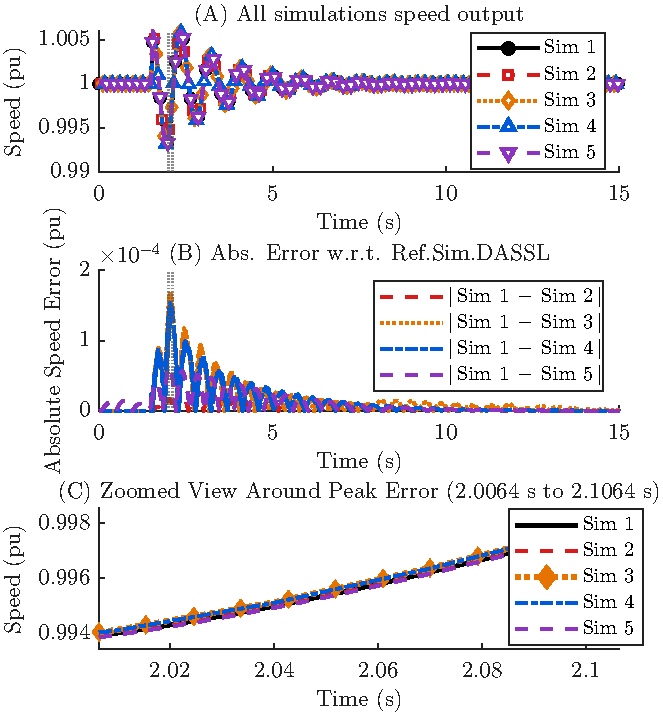
\includegraphics[width=0.95\columnwidth]{./figures/sec03_fig4_all_cases_vs_baseline.pdf}}
    \vspace{-2ex}
    \caption{MiL Simulations: (A) \texttt{w} for all simulations (see Figure \ref{fig:genunit}~(D)), (B) $\forall{i}\in\{2,3,4,5\}:\;\left|\right.$\texttt{Ref.Sim.DASSL}$\;-\;$Case$\;i\left.\right|$, (C) Zoomed view around peak error.}
    \label{fig:milsims}
    \vspace{-2ex}
\end{figure}

\begin{table}[t!]
    \centering
    \caption{Generator speed error relative to \texttt{Ref.Sim.DASSL}.}
    \vspace{-2ex}
    \label{tab:milstats}
    \small
\begin{tabular}{@{} c S[table-format=1.4e-1] S[table-format=1.4e-1] c @{}}
\toprule
Case & {max $|\epsilon|$ (pu)} & {RMS $\epsilon$ (pu)} & {$t_{\max}$ (s)} \\ \midrule
2    & 3.0160e-05            & 9.2302e-06            & 3.2156           \\
3    & 1.6949e-04            & 3.0662e-05            & 2.0564           \\
4    & 1.5353e-04            & 2.7456e-05            & 2.0564           \\
5    & 6.1989e-05            & 1.6466e-05            & 2.0310           \\ \bottomrule
\end{tabular}
    \vspace{-2ex}
\end{table}

The subsequent step to further refine the level of detail in our representation of the CHiL configuration is to generate eFMUs for \emph{both} the \controller{} \emph{and} the \plant{}, and then employ these in place of the \texttt{pss} and \texttt{G4CHIL} models as illustrated in Figures~\ref{fig:chilmodels}(C) and (D) to conduct SiL tests of the generated eFMI production code.
